\section*{Μαθηματικοί Ορισμοί}
\addcontentsline{toc}{section}{Μαθηματικοί Ορισμοί}
\newtheorem{definition}{Ορισμός}
\label{appendix:math_definitions}

\begin{definition}[Συνάρτηση argmax]
\label{definition:argmax}
Δεδομένων ενός τυχαίου συνόλου \(X\), ενός συνόλου \(Y\) και μιας συνάρτησης \(f: X\rightarrow Y\), το μέγιστο όρισμα, argmax, πάνω σε ένα υποσύνολο \(S \subseteq X\) ορίζεται ως
\[argmax_{S} \: f := \underset{x \in S}{argmax} f(x) := \{x \in S \: | \: f(s) \leq f(x)  \: \forall s \in S\} \]

Με άλλα λόγια, η συνάρτηση argmax είναι το σύνολο των σημείων \(x\) για τα οποία η \(f(x)\) παίρνει την μέγιστη τιμή της.
\end{definition}

\begin{figure}[h]
\centering
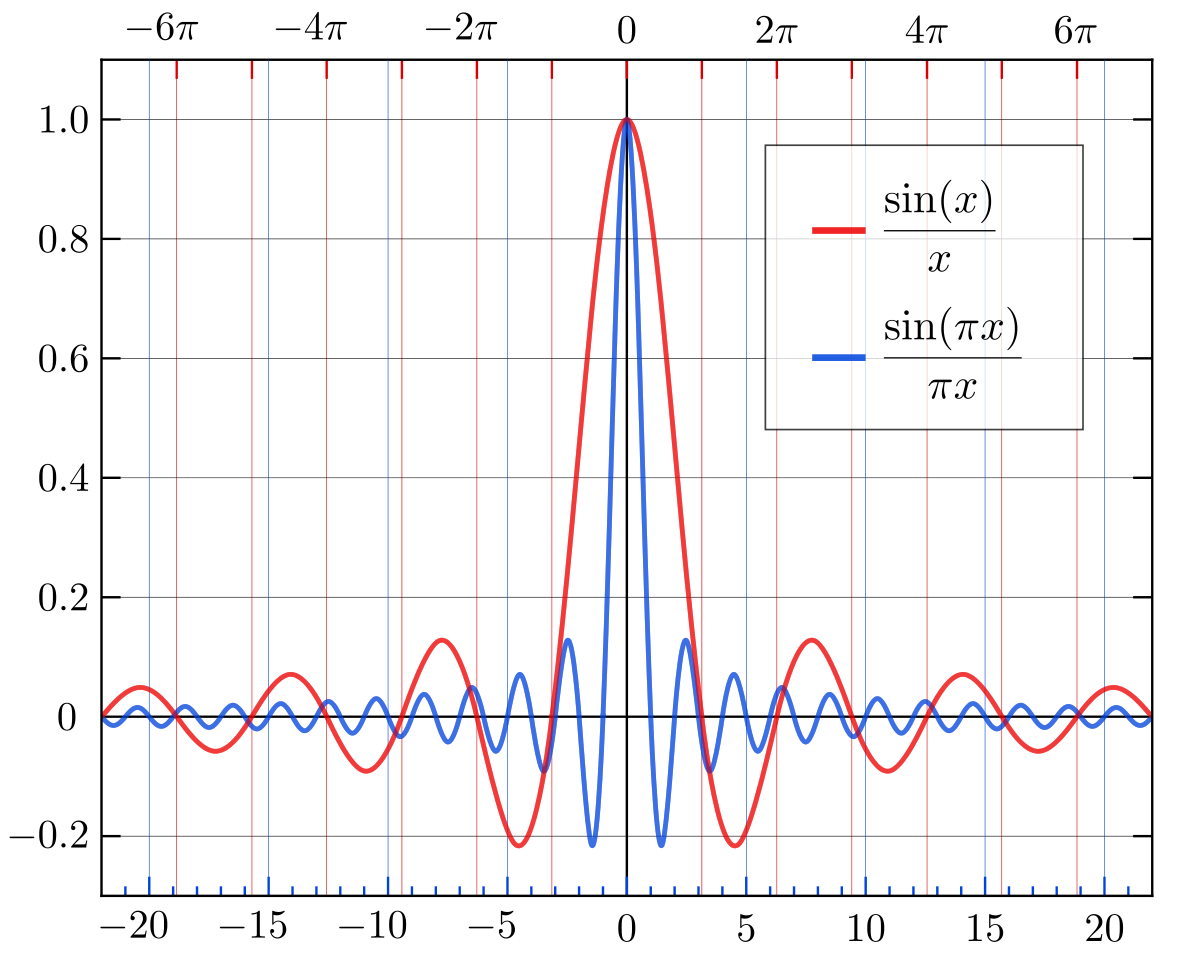
\includegraphics[scale=0.2]{images/appendix/function_argmax_example.png}
\caption[Παράδειγμα συνάρτησης argmax]{Για παράδειγμα, οι συναρτήσεις \(sinc\) της γραφικής παράστασης έχουν και οι δύο \(argmax = 0\) επειδή έχουν μέγιστο το 1 στο \(x = 0\). }
\end{figure}

\begin{definition}[Συνάρτηση soft-argmax]
\label{definition:soft-argmax}
Η συνάρτηση soft-argmax \(f: \mathbb{R}^K  \rightarrow [0, 1)^K\) ορίζεται όταν \(\lVert K \rVert > 1\) ως

\(soft\_argmax = \sigma(\boldsymbol{x})_i := \frac{e^{x_i}}{\sum_{j=1}^{K}e^{x_j}}\) για \(i = 1,\cdots,K\) και \(\boldsymbol{x} = (x_1,\cdots,x_K) \in \mathbb{R}^K \)

\end{definition}

Ουσιαστικά, η συνάρτηση soft-argmax εφαρμόζει την κανονική εκθετική συνάρτηση σε κάθε στοιχείο \(x_i\) του διανύσματος \(\boldsymbol{x}\) και κανονικοποιεί τις τιμές διαιρώντας με το άθροισμα όλων των εκθετικών. Η κανονικοποίηση αυτή εξασφαλίζει ότι το άθροισμα των στοιχείων του διανύσματος εξόδου \(\sigma(\boldsymbol{x})\) είναι 1.

\begin{definition}[Συνάρτηση ReLU]
\label{definition:relu}
Η συνάρτηση ReLU \(f: \mathbb{R} \rightarrow \mathbb{R}^+ \) ορίζεται ως

\( f(x) = max(0, x) \)

\end{definition}

Έχει ως έξοδο το όρισμα της όταν \(x > 0\), ενώ όταν \(x \leq 0\) η έξοδος είναι 0.

\begin{figure}[h]
\centering
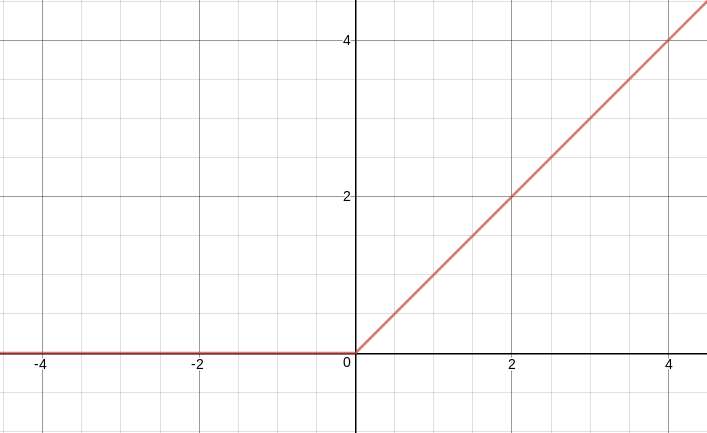
\includegraphics[scale=0.5]{images/appendix/relu_function.png}
\caption{H συνάρτηση ReLU}
\end{figure}
